\subsection{Web Klijent}
Web klijent implementiran kao dio ovog rada služi isključivo kao primjer, ideja je da se zbog izbora formata videa 
može jednostavno integrirati sa sustavom neovisno o platformi. \\
Sve što je potrebno za integraciju je video player koji podržava \foreign{webm} kontejner i \foreign{vp9} kodek.
\paraBreak
Sam klijent je vrlo jednostavan, sastoji se od forme za prijavu te prikaza svih trenutno spojenih kamera

\subsubsection{Autentifikacija}
Nakon što korisnik unese korisničko ime i lozinku šalje se zahtjev na poslužitelj koji u slučaju korektno poslanih
podataka odgovara s JWT tokenom \ref{sec:jwt}, zatim je korisnik preusmjeren na stranicu prikaza prijenosa.

\begin{figure} [h]
  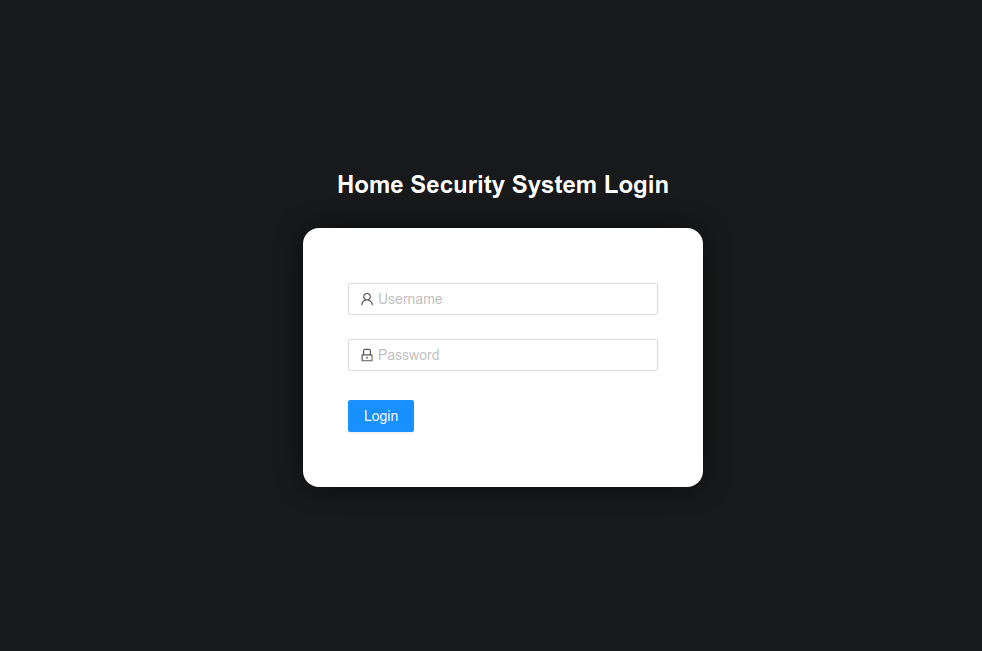
\includegraphics[width=\textwidth]{web_login.png}
  \caption{Forma za prijavu}
\end{figure}

\subsubsection{Prikaz živih prijenosa}
Prvi korak u prikazu prijenosa je zahtjev na poslužitelj za dohvat liste svih dostupnih kamera i njihovih identifikatora. 
Ovaj zahtjev očekuje \foreign{JWT} token u \foreign{Authorization} zaglavlju samog zahtjeva.
\\
Odgovor poslužitelja predstavlja popis svih kamera u obliku \foreign{array-a}, za svaku od kamera kreira se \foreign{HTML} 
video element kojem se izvor postavi na odgovarajuću rutu za gledanje \ref{sec:routes} ovisno o identifikatoru kamere

\begin{figure}[h]
  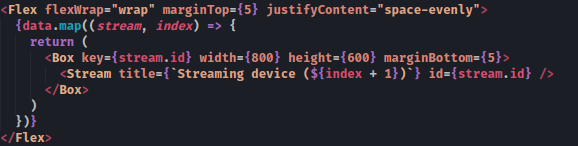
\includegraphics[width=\textwidth]{react_stream_list_comp.png}
  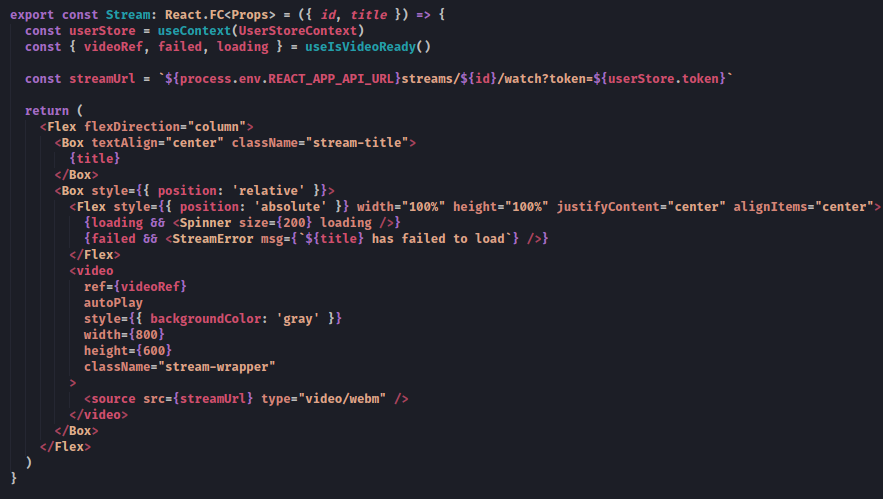
\includegraphics[width=\textwidth]{react_stream_comp.png}
  \caption{Implementacija u react-u}
\end{figure}

\begin{figure} [h]
  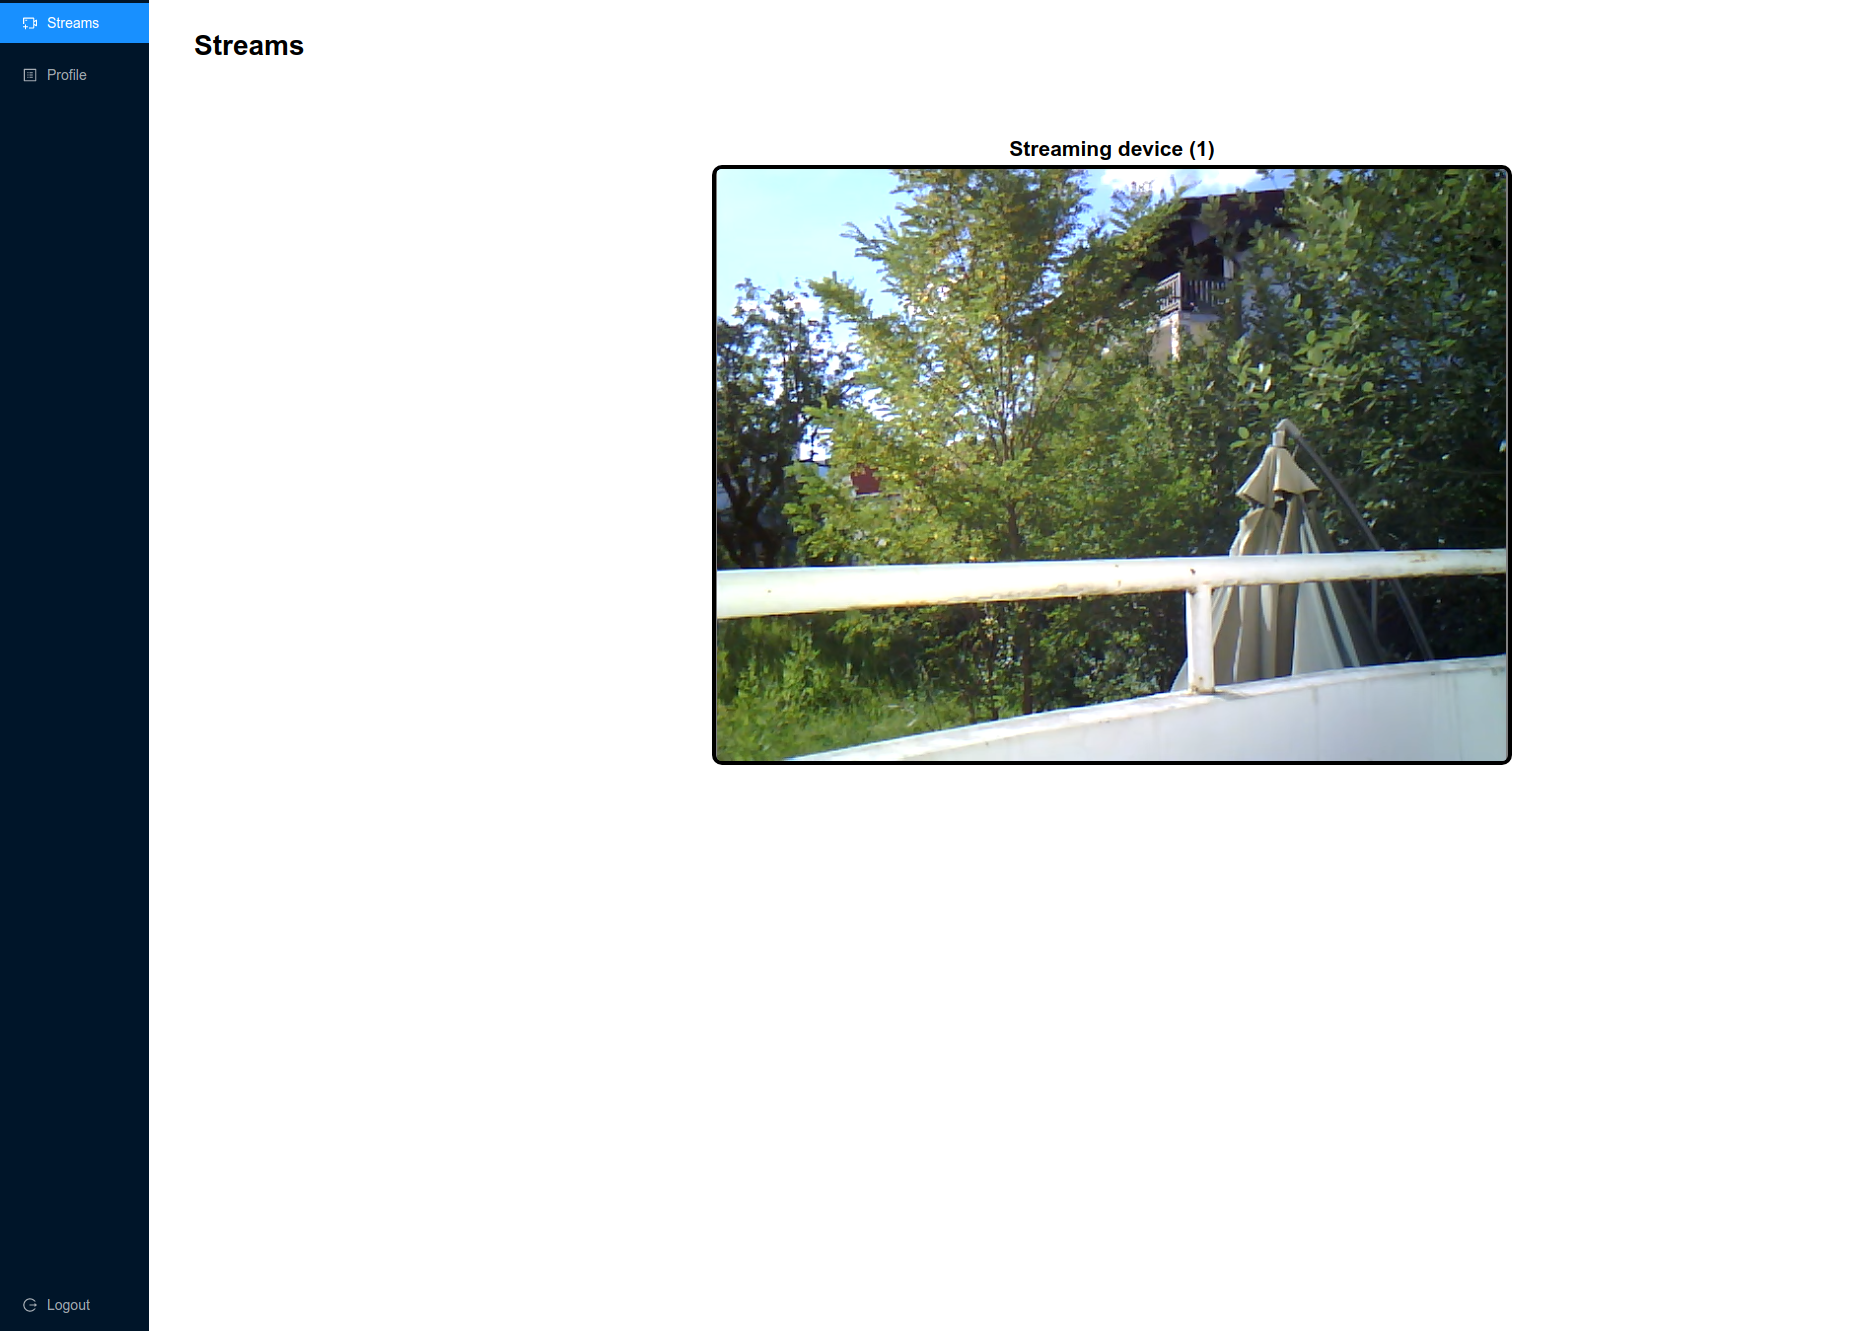
\includegraphics[width=\textwidth]{web_client1.png}
  \caption{Prikaz živih prijenosa}
\end{figure}

\begin{figure} [h]
  
\includegraphics[width=\textwidth]{web_no_streams.png}
  \caption{Nema dostupnih prijenosa}
\end{figure}

\begin{figure} [h]
  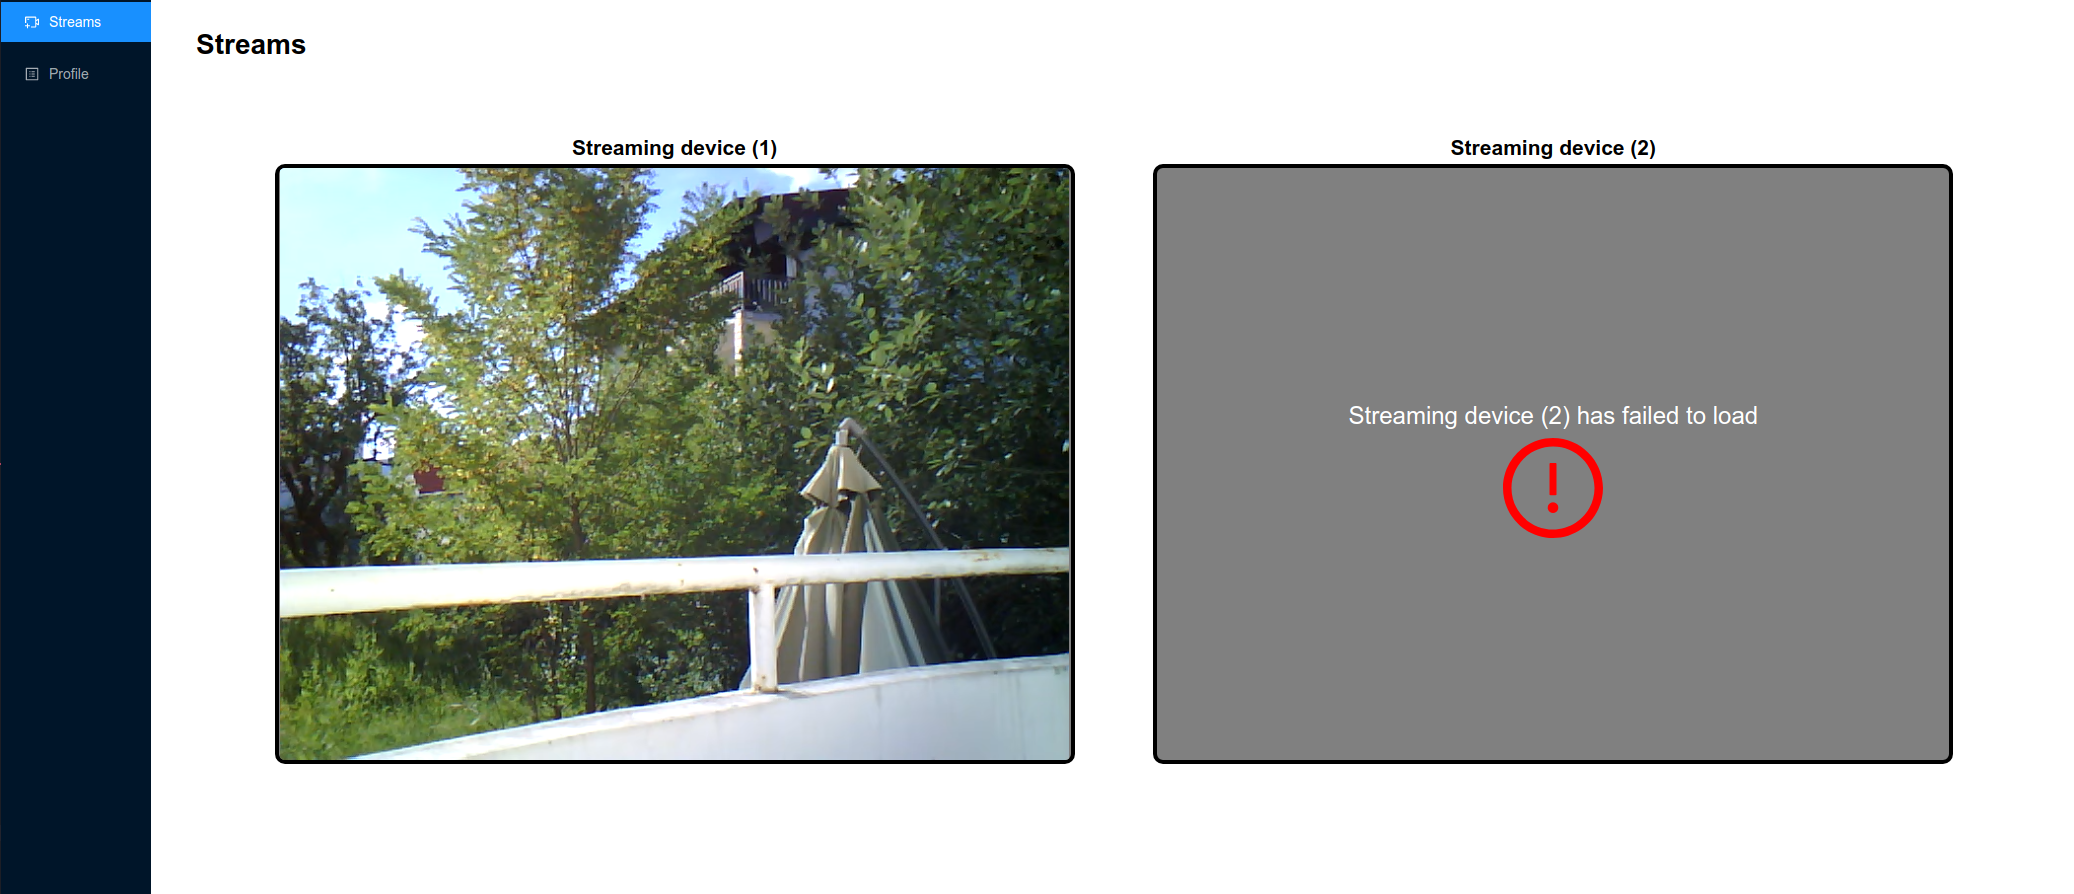
\includegraphics[width=\textwidth]{web_client_invalid_stream.png}
  \caption{Greška tijekom dohvaćanja živog prijenosa}
\end{figure}

\begin{figure} [h]
  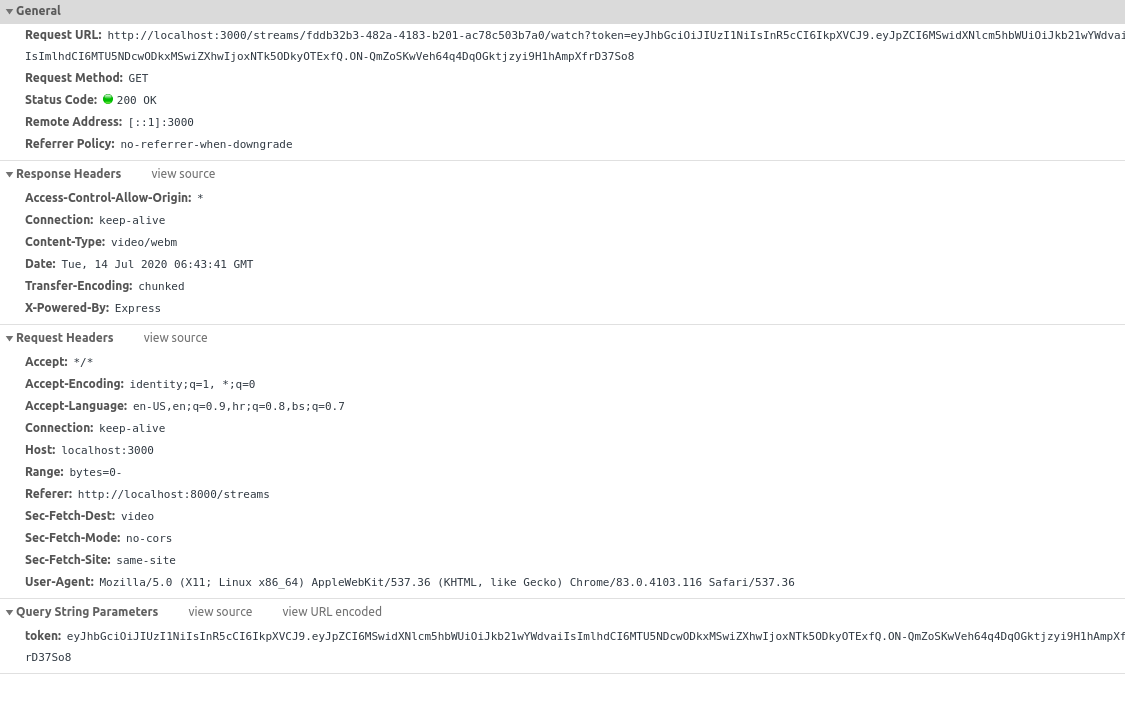
\includegraphics[width=\textwidth]{watch_request.png}
  \caption{Zahtjev za prijenos}
\end{figure}
